\documentclass{ximera}

\usepackage{microtype}
\usepackage{tikz}
\usepackage{tkz-euclide}
\usetkzobj{all}
\tikzstyle geometryDiagrams=[ultra thick,color=blue!50!black]

\renewcommand{\epsilon}{\varepsilon}



\title{Lines, angles, and areas in stereographic projection}
\begin{document}
\begin{abstract}
Here we look at lines, angles, and areas in central
projection coordinates.
\end{abstract}
\maketitle


\section{Stereographic projection sends lines to circles (or lines)}

As we know, we cannot make perfect flat maps of 3D-surfaces. In
stereographic projection, shortest paths are sent to either lines or
circles, and perhaps surprisingly, circles are sent to circles!



\begin{problem}
  Show that ``lines'' in $K$-geometry correspond to either lines or
  circles in $(x_{s},y_{s})$-coordinates under stereographic
  projection.

\begin{hint}
  To intersect two surfaces, say $f(x,y,z)=a$ and $g(x,y,z)=b$,
  simply examine
  \[
  f(x,y,z)-g(x,y,z) = a-b.
  \]
\end{hint}

\begin{hint}
  Explain why intersecting the $K$-surface
  \[
  1 = K\left(x^2+y^2\right) + z^2 
  \]
  with the plane
  \[
  ax+by+cz = 0
  \]
  produces a $K$-geometry line.
\end{hint}

\begin{hint}
  Use the projection formulas
  \begin{align*}
      x &= \frac{4x_s}{K\left(x_s^2 + y_s^2\right) + 4},\\
      y &= \frac{4y_s}{K\left(x_s^2 + y_s^2\right) + 4},\\
      z &= \frac{4-K\left(x_s^2 + y_s^2\right)}{4+K\left(x_s^2 + y_s^2\right)},
  \end{align*}
  and note that these points are \textit{necessarily} on the surface
  \[
  1 = K\left(x^2+y^2\right) + z^2.
  \]
\end{hint}

\begin{hint}
  If $c=0$, then you will find the line
  \[
   ax_s + by_s = 0.
  \]
\end{hint}

\begin{hint}
  If $c\ne 0$, then you will find the circle
  \[
   \left(x_s - \frac{2a}{cK}\right)^2 + \left(y_s -
   \frac{2b}{cK}\right)^2 = \frac{4a^2 + 4b^2 + 4c^2K}{(cK)^2}.
   \]
   You will need to complete the square to find it in this form.
\end{hint}

\begin{freeResponse}
  Let's start by intersecting the surfaces
  \[
  K\left(x^2+y^2\right)+z^2=1\qquad\text{and}\qquad ax+by+cz=0,
  \]
  where the latter is a plane passing through the origin. Write
  \[
  K\left(x^2+y^2\right) + z^2- ax- by-cz=1.
  \]
  Now use the projection formulas. Since these formula necessarily
  produce points on the surface
  \[
  1 = K\left(x^2+y^2\right) + z^2,
  \]
  we may replace $K\left(x^2+y^2\right) + z^2$ with $1$ and write
\begin{align*}
1-\frac{4ax_s}{K\left(x_s^2 + y_s^2\right) + 4}- \frac{4by_s}{K\left(x_s^2 + y_s^2\right) + 4}-c\frac{4-K\left(x_s^2 + y_s^2\right)}{4+K\left(x_s^2 + y_s^2\right)}&=1\\
 -\frac{4ax_s}{K\left(x_s^2 + y_s^2\right) + 4}- \frac{4by_s}{K\left(x_s^2 + y_s^2\right) + 4}-c\frac{4-K\left(x_s^2 + y_s^2\right)}{4+K\left(x_s^2 + y_s^2\right)}&=0.
\end{align*}
Since $K\left(x_s^2 + y_s^2\right) + 4 \ne 0$, we may clear
denominators to find 
  \begin{align*}
    -4ax_s-4by_s-4c + cK\left(x_s^2+y_s^2\right) &= 0\\
    cKx_s^2-4ax_s + cKy_s^2-4by_s-4c &= 0.
  \end{align*}
  At this point, note if $c=0$, then our equation becomes
  \begin{align*}
    -4ax_s -4by_s &= 0\\
    ax_s + by_s &= 0,
  \end{align*}
  and this is the equation for a line. Now assume that $c\ne 0$ and
  complete the square(s)
  \begin{align*}
  \left(cKx_s^2 - 4ax_s + \frac{4a^2}{cK}\right) + \left(cKy_s^2 - 4by_s + \frac{4b^2}{cK}\right) &=
  \frac{4a^2}{cK} + \frac{4b^2}{cK} + 4c\\
  \left(x_s\sqrt{cK} - \frac{2a}{\sqrt{cK}}\right)^2 + \left(y_s\sqrt{cK} - \frac{2b}{\sqrt{cK}}\right)^2&=\frac{4a^2}{cK} + \frac{4b^2}{cK} + 4c.
  \end{align*}
  Multiply through by $(cK)^{-1/4}$ to find
  \begin{align*}
    \left(x_s - \frac{2a}{cK}\right)^2 + \left(y_s - \frac{2b}{cK}\right)^2 &= \frac{4a^2}{(cK)^2} + \frac{4b^2}{(cK)^2} + \frac{4c}{cK}\\
    \left(x_s - \frac{2a}{cK}\right)^2 + \left(y_s - \frac{2b}{cK}\right)^2 &= \frac{4a^2 + 4b^2 + 4c^2K}{(cK)^2}.
  \end{align*}
  This is the equation of a circle with center
  \[
  \left(\frac{2a}{cK}, \frac{2b}{cK}\right)
  \]
  and radius
  \[
  \sqrt{\frac{4a^2 + 4b^2 + 4c^2K}{(cK)^2}}.
  \]
\end{freeResponse}
\end{problem}



\begin{remark}
  With entirely similar reasoning, you can show that circles in
  stereographic projection are also sent to either circles (or lines).
\end{remark}


When we project shortest paths, they map to circles (unless $c=0$ as
above). When $K<0$, the circles meet the ``circle at infinity'' at right angles. 

\begin{image}
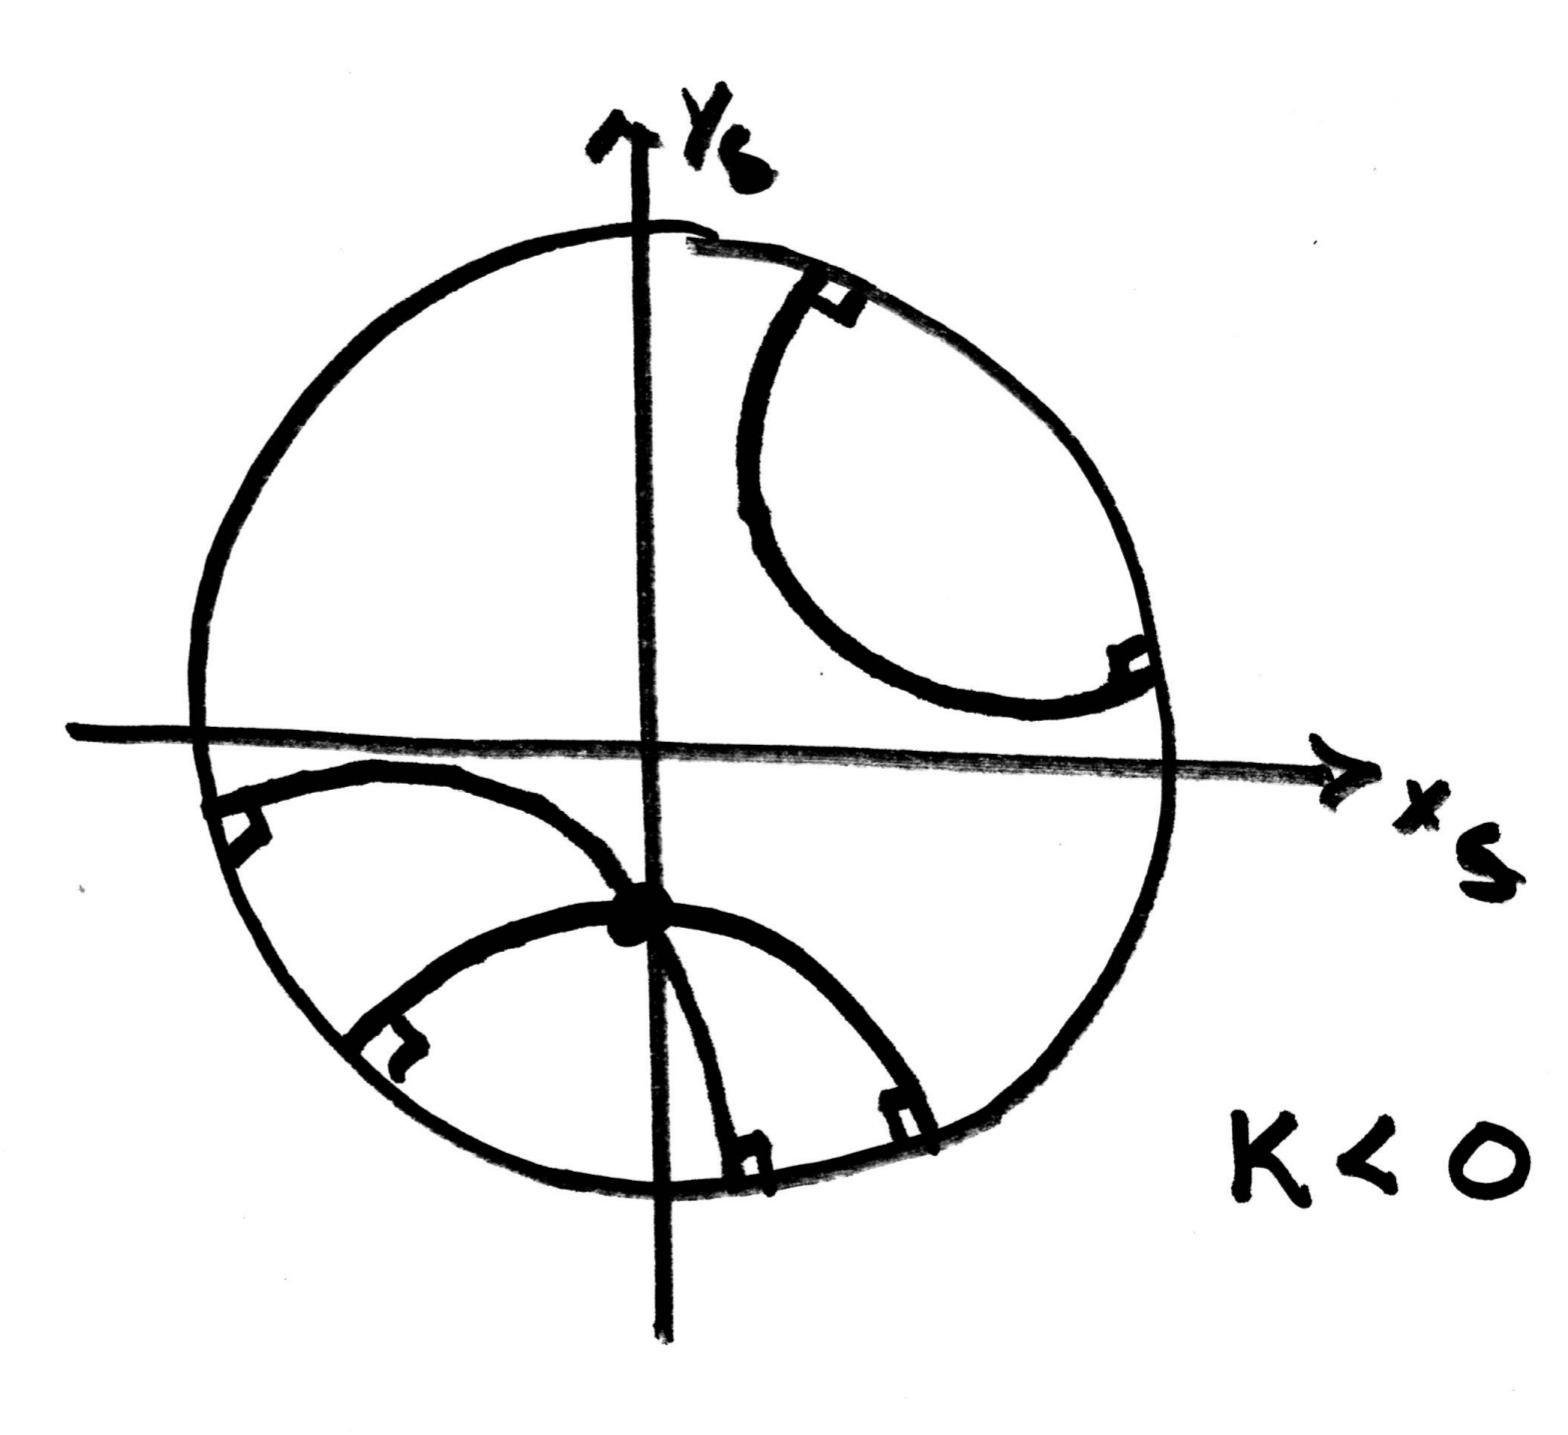
\includegraphics[width=3in]{stereoLines.png}
\end{image}

\begin{problem}
  If $K<0$ explain why Euclid's fifth axiom:
  \begin{quote}
    Through a point not on a line there passes a unique parallel line.
  \end{quote}
  fails.
  \begin{freeResponse}
    Given a point not on a line, we see that there are many lines
    parallel to the original line through that point.
  \end{freeResponse}
\end{problem}







\section{Stereographic projection preserves angles}


A remarkable fact about stereographic projection is that it
``preserves'' angles. This means that the angles we see in
stereographic projection are true representations of the angle in
euclidean coordinates.  Now that we are masters of dot products, we
will prove this fact with ease!

\begin{problem}
  Show that
  \[
  \frac{V_s\bullet_s W_s}{|V_s|_s\cdot|W_s|_s} = \frac{V_s\bullet W_s}{|V_s|\cdot|W_s|}.
  \]
  \begin{hint}
    On the right-hand side we are using the euclidean dot product and
    euclidean length formula.
  \end{hint}
    \begin{freeResponse}
    Let
      \[
      V_s=
      \begin{bmatrix}
        a & b
      \end{bmatrix}
      \qquad\text{and}\qquad
      W_s=
      \begin{bmatrix}
        c & d
      \end{bmatrix}.
      \]
      Write
      \begin{align*}
        \frac{V_s\bullet_s W_s}{|V_s|_s\cdot|W_s|_s} &= \frac{
          \begin{bmatrix}
            a & b
          \end{bmatrix}
          \begin{bmatrix}
            \rho^2 & 0 \\
            0 & \rho^2
          \end{bmatrix}
          \begin{bmatrix}
            c\\
            d
          \end{bmatrix}
        }{
          \sqrt{\begin{bmatrix}
            a & b
          \end{bmatrix}
          \begin{bmatrix}
            \rho^2 & 0 \\
            0 & \rho^2
          \end{bmatrix}
          \begin{bmatrix}
            a\\
            b
          \end{bmatrix}}
          \cdot
          \sqrt{\begin{bmatrix}
            c & d
          \end{bmatrix}
          \begin{bmatrix}
            \rho^2 & 0 \\
            0 & \rho^2
          \end{bmatrix}
          \begin{bmatrix}
            c\\
            d
          \end{bmatrix}}
        }\\
        &= \frac{ac\rho^2 + bd\rho^2}{\sqrt{a^2\rho^2+b^2\rho^2}\cdot \sqrt{c^2\rho^2+d^2\rho^2}}\\
        &= \frac{\rho^2(ac + bd)}{\rho^2\sqrt{a^2+b^2}\cdot \sqrt{c^2+d^2}}\\
        &= \frac{ac + bd}{\sqrt{a^2+b^2}\cdot \sqrt{c^2+d^2}}\\
        &=\frac{V_s\bullet W_s}{|V_s|\cdot|W_s|}.
    \end{align*}
  \end{freeResponse}
\end{problem}


\begin{problem}
  Explain how the last problem shows that stereographic projection
  ``preserves'' angles. 
\end{problem}




%% \begin{problem}
%% Draw a picture of an angle between two paths through a point on
%%   the Euclidean $R$-sphere and the stereographic projection of that
%%   angle onto the plane $\hat{z}=R$. Try to give an intuitive geometric
%%   explanation for why it should have the same measure as the original
%%   angle.
%% \end{problem}
















\section{Areas in stereographic projection coordinates}

Let's use the power of stereographic coordinates to compute the areas
of spherical, hyperbolic, and euclidean circles.

We know that the area of a region in stereographic coordinates is given by 
\[
\int_{C_s} \sqrt{
  \det
  \begin{bmatrix}
    \dd[X]{x_s}\bullet_K \dd[X]{x_s} & \dd[X]{y_s}\bullet_K \dd[X]{x_s} \\
    \dd[X]{x_s}\bullet_K \dd[X]{y_s} & \dd[X]{y_s}\bullet_K \dd[X]{y_s}
  \end{bmatrix}
}\d x_s\d y_s
\]

\begin{problem}
  Give a heuristic explanation of why this integral computes what we
  say it computes.
\end{problem}

You have already shown that
\[
\int_{C_s} \sqrt{
  \det
  \begin{bmatrix}
    \dd[X]{x_s}\bullet_K \dd[X]{x_s} & \dd[X]{y_s}\bullet_K \dd[X]{x_s} \\
    \dd[X]{x_s}\bullet_K \dd[X]{y_s} & \dd[X]{y_s}\bullet_K \dd[X]{y_s}
  \end{bmatrix}
}\d x_s\d y_s
\]
\[
=
\int_{C_s} \sqrt{
  \det\left(
  \begin{bmatrix}
    \dd[X]{x_s}\\
    \dd[X]{y_s}
  \end{bmatrix}
  \begin{bmatrix}
    1 & 0 & 0\\
    0 & 1 & 0\\
    0 & 0 & K^{-1}
  \end{bmatrix}
  \begin{bmatrix}
    \left(\dd[X]{x_s}\right)^\transpose & \left(\dd[X]{y_s}\right)^\transpose
  \end{bmatrix}\right)
}\d x_s\d y_s
\]

\begin{problem}
  Explain why
  \[
\begin{bmatrix}
    \dd[X]{x_s}\\
    \dd[X]{y_s}
  \end{bmatrix}
  \begin{bmatrix}
    1 & 0 & 0\\
    0 & 1 & 0\\
    0 & 0 & K^{-1}
  \end{bmatrix}
  \begin{bmatrix}
    \left(\dd[X]{x_s}\right)^\transpose & \left(\dd[X]{y_s}\right)^\transpose
  \end{bmatrix} =P_s.
  \]
  \begin{hint}
    No new computations need to be done, just look at how $P_s$ was derived.
  \end{hint}
\end{problem}

Hence now we see 
\[
\int_{C_s} \sqrt{
  \det
  \begin{bmatrix}
    \dd[X]{x_s}\bullet_K \dd[X]{x_s} & \dd[X]{y_s}\bullet_K \dd[X]{x_s} \\
    \dd[X]{x_s}\bullet_K \dd[X]{y_s} & \dd[X]{y_s}\bullet_K \dd[X]{y_s}
  \end{bmatrix}
}\d x_s\d y_s = \int_{C_s} \sqrt{\det P_s}\d x_s\d y_s
\]

\begin{problem}
  Compute $\sqrt{\det P_s}$ in terms of $K$, $x_s$, and $y_s$.
\end{problem}


\begin{problem}
  Examining the following diagram
  \begin{image}
    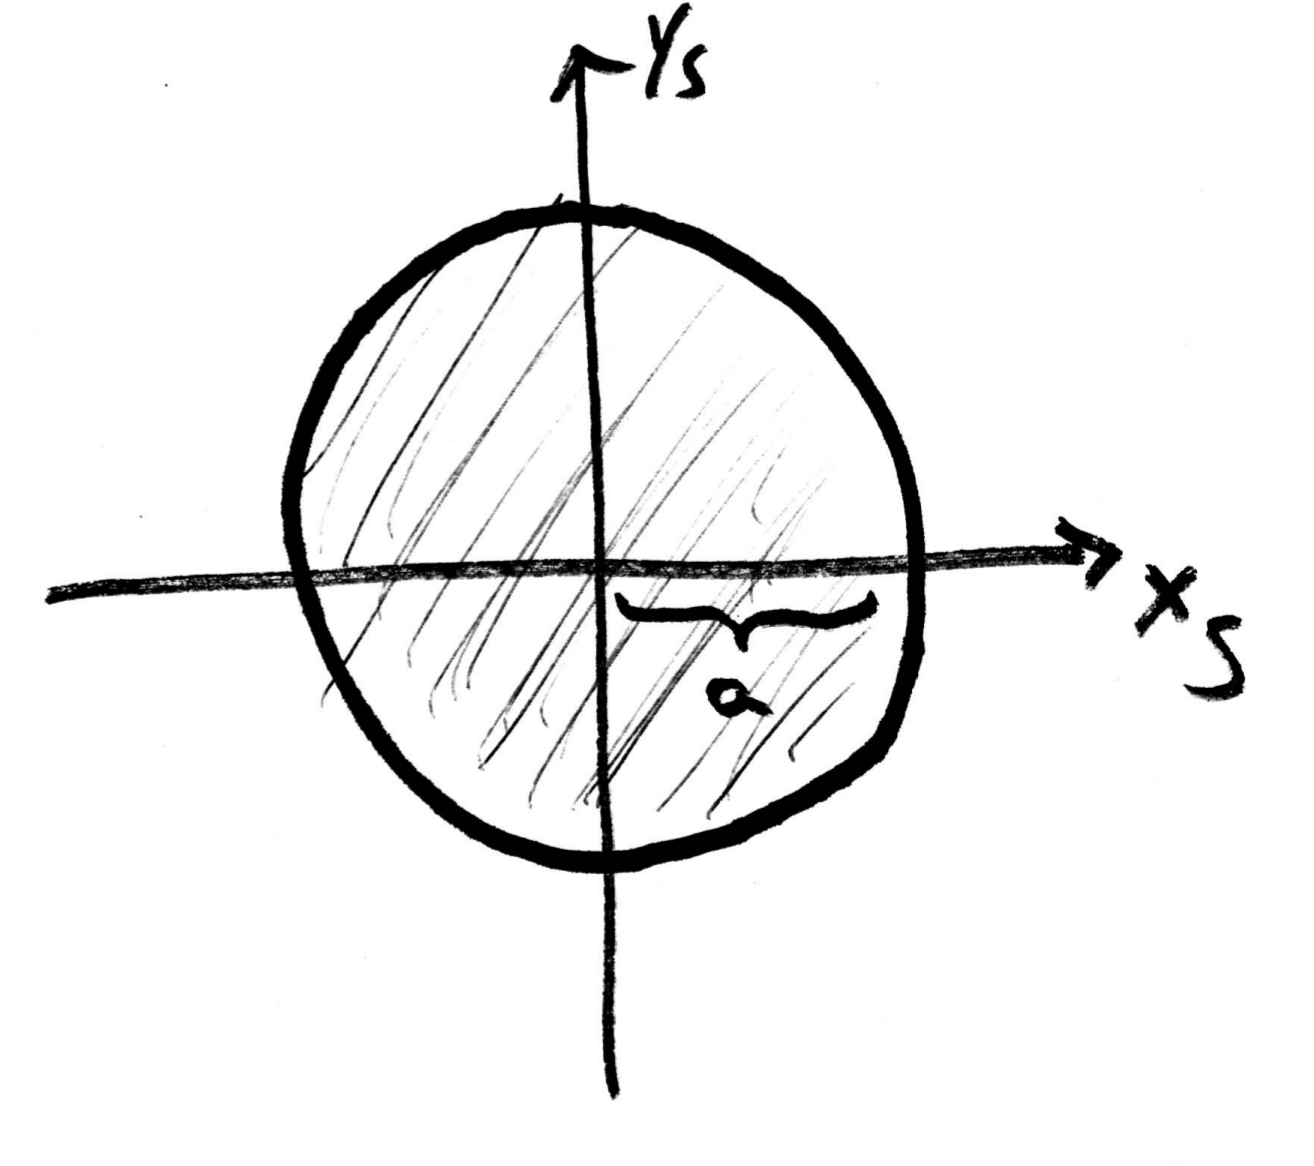
\includegraphics[width=3in]{stereoCirc.png}
  \end{image}
  convert
  \[
  \int_{C_s} \frac{16}{\left(K\left(x_s^2+y_s^2\right)+4\right)^2} \d x_s\d y_s.
  \]
  to polar coordinates and compute the integral.
  \begin{hint}
    Recall that to covert to polar coordinates, set
    \begin{align*}
      r &= \sqrt{x_s^2+y_s^2},\\
      \theta &= \arctan(y_s/x_s),
    \end{align*}
    and replace $\d x_s\d y_s$ with $r\d r\d \theta$.
  \end{hint}
  \begin{freeResponse}
    \[
    \int_{C_s} \frac{16}{\left(K\left(x_s^2+y_s^2\right)+4\right)^2} \d x_s\d y_s
    = \int_0^{2\pi} \int_0^a \frac{16}{\left(K\cdot r^2+4\right)^2} r\d r \d \theta.
    \]
    Integrating this from the inside-out we find
    \begin{align*}
      \int_0^{2\pi} \int_0^a \frac{16}{\left(K\cdot r^2+4\right)^2} r\d r \d \theta
      &= \int_0^{2\pi} \eval{\frac{-8}{K\left(K\cdot r^2+4\right)}}_0^a \d \theta\\
      &= \int_0^{2\pi} \frac{-8}{K\left(K\cdot a^2+4\right)}+\frac{2}{K} \d \theta\\
      &= \frac{4\pi}{K}-\frac{16\pi}{K\left(K\cdot a^2+4\right)}.   
    \end{align*}
  \end{freeResponse}
\end{problem}


\begin{problem}
  Compute
  \[
  \lim_{K\to 0} \left(\frac{4\pi}{K}-\frac{16\pi}{K\left(K\cdot a^2+4\right)}\right)
  \]
  and explain why your answer makes perfect sense.
  \begin{hint}
    Express this as a single fraction.
  \end{hint}
  \begin{freeResponse}
    \begin{align*}
    \lim_{K\to 0} \left(\frac{4\pi}{K}-\frac{16\pi}{K\left(K\cdot a^2+4\right)}\right)
    &= \lim_{K\to 0} \left(\frac{4\pi\left(K\cdot a^2+4\right) - 16\pi}{K\left(K\cdot a^2+4\right)}\right)\\
    &= \lim_{K\to 0} \left(\frac{4\pi K\cdot a^2}{K\left(K\cdot a^2+4\right)}\right)\\
    &= \lim_{K\to 0} \left(\frac{4\pi\cdot a^2}{K\cdot a^2+4}\right)\\
    &= \frac{4\pi\cdot a^2}{4}\\
    &= \pi\cdot a^2.\\
    \end{align*}
    This makes perfect sense because when $K=0$, we are in the
    euclidean plane. Hence the area of the circle is $\pi\cdot a^2$.
  \end{freeResponse}
\end{problem}




\section{Stereographic projection unifies euclidean, spherical, and hyperbolic geometry}


Under stereographic projection, our new dot product defined by
\[
V_s\bullet_s W_s = V_s\cdot P_s\cdot W_s^\transpose
\]
make sense when $K$ is zero, positive, and negative. Hence this dot
product makes sense for euclidean, spherical, and hyperbolic
geometry. However, in stereographic projection, shortest paths on the
$K$-surface
\[
K\left(x^2 + y^2\right) + z^2 = 1
\]
map to circles (or lines) in the plane $z=1$. The advantage of
stereographic projection over central projection is that angles are
preserved in stereographic projection. This means that when angles are
projected into the plane via stereographic projection, the angle we
see in the $(x_s,y_s)$-plane is the actual angle between two
vectors. Summarizing, we have:




\[
{\renewcommand{\arraystretch}{2.7}
  \begin{array}{|c||c|c|c|}\hline
    & \text{Spherical} (K>0) & \text{Euclidean} (K=0) & \text{Hyperbolic} (K<0)\\\hline\hline
    \text{Surface in} \\ \text{euclidean space} & \hat{x}^{2}+\hat{y}^{2}+\hat{z}^{2}=R^{2} & \text{DNE}  & \text{DNE} \\\hline
    \text{Euclidean dot product} & \hat{V}\cdot \hat{W}^\transpose & \text{DNE}  & \text{DNE}\\\hline
     \text{Surface in} K \text{-warped space} & \multicolumn{3}{c|}{1=K\left(  x^{2}+y^{2}\right)  +z^{2}}\\\hline
     K\text{-dot product} & V\left[\begin{smallmatrix}1 & 0 & 0\\ 0 & 1 & 0\\ 0 & 0 & K^{-1}\end{smallmatrix}\right] W^\transpose &  \text{DNE} & V\left[\begin{smallmatrix}1 & 0 & 0\\ 0 & 1 & 0\\ 0 & 0 & K^{-1}\end{smallmatrix}\right]W^\transpose\\\hline
     \text{Central dot product} & \multicolumn{3}{c|}{V_c\cdot P_c\cdot W_c^\transpose = V_c\left[\begin{smallmatrix}\left(Ky_c^2+1\right)\lambda^4 & -Kx_{c}y_{c}\lambda^4\\
           -Kx_{c}y_{c}\lambda^4 & \left(Kx_c^2+1\right)\lambda^4\end{smallmatrix}\right] W_c^\transpose}\\\hline
     \text{Stereographic dot product} & \multicolumn{3}{c|}{V_s\cdot P_s\cdot W_s^\transpose = V_s\left[\begin{smallmatrix}\rho^2 & 0\\
    0 & \rho^2 \end{smallmatrix}\right] W_s^\transpose}\\\hline
\end{array}}
\]





\begin{problem}
Summarize the results from this section. In particular, indicate which
results follow from the others.
\begin{freeResponse}
\end{freeResponse}
\end{problem}


\end{document}
